\section{RL basics}
Firstly, environment where an agent is able to operate must be defined. Environment can be described as Markov decision process, where $S_t \in \mathcal{S}$ is a state from a set of possible states $\mathcal{S}$ in which environment is located in time $t$. Agent can usually observe the state of the environment and take action accordingly. Action is a probabilistic transition between states. Every action $A_t \in \mathcal{A}$ moves the environment from $S_t$ to $S_{t+1}$. The environment evaluates every action and returns appropriate reward $R_t$ (figure 1). In RL set $\mathcal{A}$ is often called action space and set $\mathcal{S}$ observation space. The main goal of the agent is to find policy $\pi$ which maximises expected return. Return $G_t$ is a sum of discounted future rewards \cite{sutton2012}.
\begin{equation}
G_t = \sum\limits_{k=0}^{\infty}\gamma^k R_{t+k}
\end{equation}
where $\gamma \in [0,1]$ is discount factor. RL methods define how experiences from interacting with environment will change the policy.  Major issue is that maximising immediate reward is often not an effective approach to maximise expected sum of discounted rewards. This greedy policy can take the agent into very disadvantageous state. Thus, the agent must take into account future states and rewards. This is done by value function $V_pi(S_t)$ which assesses how advantageous is being in state $S_t$ with policy $\pi$.
\begin{equation}
V_\pi(S_t) \doteq  \mathbf{E}_\pi[G_t | S_t].
\end{equation}
Optimal policy $\pi^*$ is then defined as
\begin{equation}
\pi^*(S_t) \doteq \max\limits_\pi V_\pi(S_t),
\end{equation}
for all $S_t \in \mathcal{S}$
In the past agents used big tables to estimate the value function. This is possible in environments with small action and observation spaces but is very memory consuming for larger environments and even impossible for continuous action or observation space. Therefore, modern methods use neural networks as function estimators.

\begin{figure}[!h]
\centering
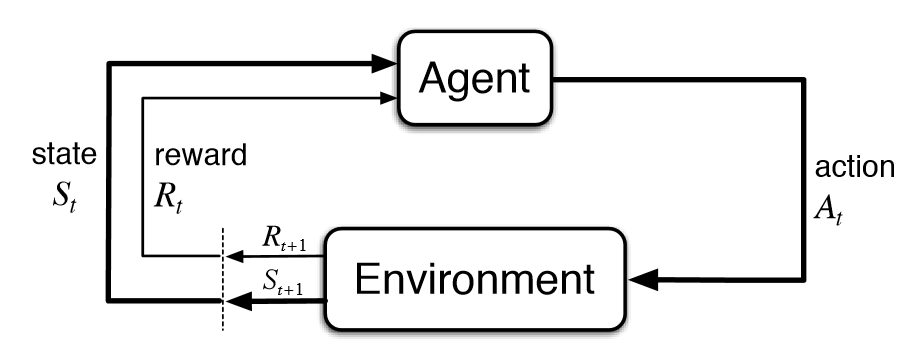
\includegraphics[scale=0.3]{fig/RL-concept.png}
\caption{RL concept}
\end{figure}

\subsection{Temporal difference learning}
Temporal difference (TD) learning combines the ideas of Monte Carlo methods and dynamic programming. It is able to learn directly from experience obtained by interactions with an environment without any prior knowledge of said environment. TD learning is done by following assignment in each timestamp \cite{sutton2012}
\begin{equation}
V(S_t) \gets V(S_t) + \alpha [R_{t} + \gamma V(S_{t+1}) - V(S_t)]
\end{equation}
where $\alpha \in \mathbb{R}^+$ is step size.

\subsection{Q-learning}
Q-learning is type of TD learning developed by Watkins \cite{watkins1992}. The state value $V$ from previous subsection is replaced by $Q$ value, which refers to quality of action in a particular state instead of quality of the state itself. When we rewrite TD learning (4) to Q-learning we get:
\begin{equation}
Q(S_t, A_t) \gets Q(S_t, A_t) + \alpha [R_{t} + \gamma \underset{A_{t+1}}{\max} Q(S_{t+1}, A_{t+1}) - Q(S_t, A_t)].
\end{equation}
Our policy here is to take action with maximal $Q$ value. That is called greedy policy. Obvious drawback of greedy policy is that it does not allow to explore the whole environment properly because an action with the highest $Q$ value is always chosen. A solution to this problem is sometimes take random action to explore the environment. This policy is often referred to as $\epsilon$-greedy policy.

\begin{algorithm}
\caption{$\epsilon$-greedy policy}\label{euclid}
\begin{algorithmic}[1]
\Procedure{ChooseAction}{}
\State $\epsilon \gets \epsilon \cdot \epsilon_d$
\If {$\epsilon >$ random $\in (0,1)$}
\State action $\gets$ random $\in \mathcal{A}$
\Else 
\State action $\gets$ $\underset{A_t}{\max} Q(S_t, A_t)$
\EndIf
\State \Return action
\EndProcedure
\end{algorithmic}
\end{algorithm}

It is common to set $\epsilon = 1$ at the beginning of the training and decay rate $\epsilon_d$ close to one. General idea behind this policy assumes that it is needed to explore an environment first and then exploit agents experience.

\clearpage
\section{Deep neural networks in RL}
As was stated in previous chapter, tabular methods are very inefficient in large environments. In these instances is possible to use deep neural networks which can replace tables. Deep Q networks (DQN) proposed by Googles Deepmind \cite{mnih2015} outperformed all previous RL algorithms in playing Atari games. With neural networks grew also the popularity of policy gradient methods where function estimator outputs an action instead of Q values. Note that the most of these methods are general and not necessarily tied to neural networks.

\subsection{Deep Q network}
Neural network takes current state as input and outputs Q value for each possible action. Network is trained using gradients of Q value in current state with respect to trainable weights $\theta$ of our neural network.
\begin{align}
\delta_t &= R_{t} + \gamma \underset{A_{t+1}}{\max}Q^\theta(S_{t+1}, A_{t+1}) - Q^\theta(S_t, A_t)\\
\theta_{t+1} &= \theta_t + \alpha \delta_t \nabla_\theta Q^\theta (S_t, A_t).
\end{align}
We are updating gradients in proportion to TD $\delta_t$. Unfortunately, this simple DQN agent suffers from a lack of sample efficiency and does not converge well. There are many techniques which can help DQNs to achieve satisfying results.

\subsection{Target network}
Target network is a technique which improves convergence of DQN learning \cite{mnih2015}. It uses two neural nets instead of one. The first is trained online network on a batch of data and the second target network is used for predictions during training. After the completion of training on a batch of data, the target network is updated
\begin{equation}
\theta^- = \tau \theta + (1-\tau)\theta^-
\end{equation}
where $\theta^-$ is set of trainable weights of the target network, $\theta$ indicates online network weights and $\tau \ll 1$ is constant.
TD $\delta$ is now calculated using target network:
\begin{equation}
\delta_t = R_{t} + \gamma \underset{A_{t+1}}{max}Q^{\theta^-}(S_{t+1}, A_{t+1}) - Q^\theta(S_t, A_t). 
\end{equation}
Target network stabilises training since predicting network does not change after each training step.

\subsection{Prioritized experience replay}
Experience replay is biologically inspired mechanism introduced by Schaul et al. \cite{schaul2015} which stores all experiences (specifically: $S_t$, $A_t$, $R_{t}$, $S_{t+1}$) into a buffer and assigns priority to every experience. Main idea is that experiences with high TD should have higher priority. It is thus necessary to calculate priority $p$ from TD error:
\begin{equation}
p = (|\delta_t | + \beta)^\rho
\end{equation}
where $\rho$ indicates how much we prefer experiences with higher priority and $\beta \ll 1$ is a constant which helps to avoid priorities very close to zero. Considering a greedy selection would abandon experiences with low priority, a better approach is to choose experience $i \in \mathcal{I}$ with probability:
\begin{equation}
P(i) = \frac{p_i}{\sum_{j \in \mathcal{I}} p_j}
\end{equation}
where $\mathcal{I}$ is set of all experiences in the buffer. It is possible now to sample a batch of experiences for training using this probability. It removes correlation in the observation sequence and improves sample efficiency of DQN. It is feasible to store all experiences in a buffer sorted by priority but a more efficient implementation is a sum tree.

\subsection{Double Q-learning}
Classic Q-learning algorithm tends to overestimate actions under certain conditions. Hasselt et al. propose idea of Double Q-learning which decompose the max operation into action selection and action evaluation \cite{hasselt2015}. TD is then computed by following equation.
\begin{equation}
\delta = R_{t} + \gamma Q^{\theta^-}(S_{t+1}, \underset{A_{t+1}}{\text{argmax}}Q^\theta(S_{t+1}, A_{t+1})) - Q^\theta (S_t, A_t).
\end{equation}
Double DQN outperforms DQN in terms of value accuracy and in terms of policy quality.

\clearpage
\section{Policy gradient}
By this section the goal of neural network was predicting values on the basis of which we determined the policy. In policy gradient method neural network approximates the policy itself. 
\begin{equation}
\theta_{t+1} = \theta_t + \alpha \widehat{\nabla J(\theta_t)}
\end{equation}
where $J$ is performance measure with respect to our neural network parameters and $\widehat{\nabla J(\theta_t)}$ is stochastic estimate which approximates gradient of performance measure. In other words, this method is basically doing stochastic gradient ascent of $J$ with respect to $\theta$ \cite{sutton1999}. Policy gradient methods are outperforming DQNs especially in continuous action spaces, because their output is directly continuous action instead of Q-value for every possible action.

\subsection{Actor-Critic}
Thanks to predicting action directly, we gain possibility to predict in continuous action space, but we lost the Q-value which assessed the advantage of action in certain state. That it why the Actor-Critic framework was created. It uses two separate neural networks - Actor which predicts action and Critic which assesses action advantage.
\begin{figure}[!h]
\centering
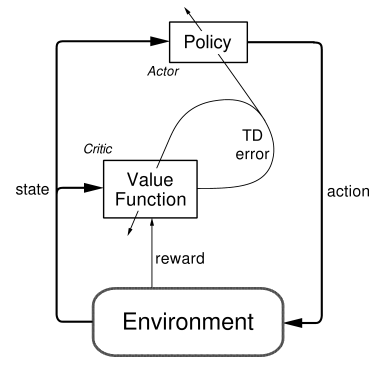
\includegraphics[scale=0.55]{fig/actor-critic.png}
\caption{Actor-Critic framework}
\end{figure}
\clearpage

\subsection{Deterministic policy gradients}
Deep deterministic policy gradient (DDPG) is one of methods exploiting the Actor-Critic framework. Before DDPG was common practice to use stochastic actor, which predicts parameters of distribution (usually normal distribution). Action of stochastic actor is then a random sample from predicted distribution. Whereas deterministic actor uses distribution sampling only for exploration of action space. We denote $\theta$ and $\omega$ for trainable weights of actor and critic, respectively. Critic update is very similar to DQN:
\begin{align}
\delta_t &= r_t + \gamma Q^\omega(S_{t+1}, \mu ^\theta (S_{t+1})) - Q^\omega(S_t, A_t)\\
\omega_{t+1} &= \omega_t + \alpha \delta_t \nabla_\omega Q^\omega(S_t, A_t).
\end{align}
Note that instead of $A_{t+1}$ is now used function $\mu^\theta(S)$, which is an action estimate by actor neural network. Actor update rule is not so straightforward. 
\begin{equation}
\theta_{t+1} = \theta_t + \alpha\nabla_\theta \mu^\theta(S_t)\nabla_a Q^\omega (S_t, A_t)|_{a = \mu^\theta(S_t)}.
\end{equation}
This equation uses chain rule for derivatives to obtain gradient of Q-values with respect to trainable weights $\theta$. Namely:
\begin{equation}
\frac{\partial Q^\omega(S_t, A_t)}{\partial \theta} = \frac{\partial Q^\omega(S_t, A_t)}{\partial A_t} \frac{\partial A_t}{\partial \theta}.
\end{equation}
DDPG significantly outperforms its stochastic counterparts, especially in big continuous action spaces \cite{silver2014}.

\subsection{Wolpetinger policy}
Actor-Critic methods and DDPG work well in continuous action spaces, but there is a lot of problems with large discrete action spaces, such as recommender systems or lidar planning. Wolpetinger policy is approach how to utilize DDPG in discrete action space \cite{dulac2015}. Actor doesn't predict action directly, but it predicts so called proto-action $\tilde{A_t}$.
\begin{equation}
\tilde{A_t} = \mu^\theta(S_t).
\end{equation}
Proto action mostly isn't valid action $\tilde{A_t} \notin \mathcal{A}$. Thus it is necessary to find valid action corresponding to proto action. This is done by computing euclidean distance to every possible action.
\begin{equation}
\mathcal{A}_{knn} = \underset{a \in \mathcal{A}}{\text{argmin}}^N | a - \tilde{A_t} |_2 .
\end{equation}
Usually policy choose $N$ closest action to the proto action. $\mathcal{A}_{knn}$ is the set of closest action to proto action. Whole set is then assessed by critic and action with highest Q-value is finally picked.
\begin{equation}
A_t = \underset{a \in \mathcal{A}_{knn}}{\text{argmax}} Q^\omega(S_t, a)
\end{equation}
\begin{figure}[!h]
\centering
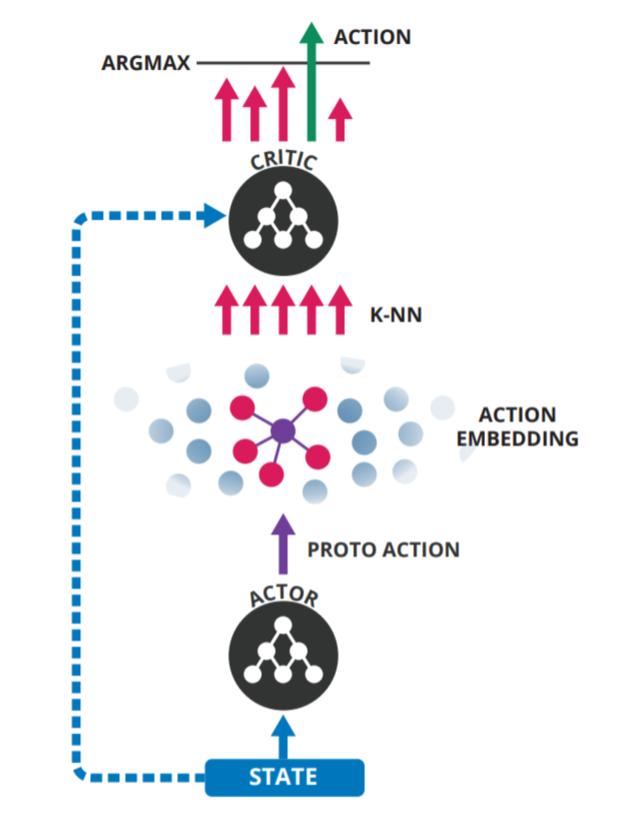
\includegraphics[scale=0.35]{fig/wolpetinger-policy.png}
\caption{Wolpetinger policy illustration}
\end{figure}

\subsection{Parameter and action space noise}
In large action space is very important to emphasize agents exploration. Bad exploration can cause that agent converges prematurely and ends up in local optimum. DDPG commonly use stochastic policy to slightly modify actors actions.
\begin{equation}
\hat{A_t} = \mu^\theta(S) + \mathcal{N}(0, \sigma^2)
\end{equation}
where $\mathcal{N}$ is normal distribution with mean value equal to zero and variance, which is reducing during the training and $\hat{A_t}$ is perturbed action. Action space noise helps agent to explore the environment. Another approach is to apply noise directly to actors weights. It can sometimes lead to more consistent exploration and richer behaviours \cite{plappert2017}.
\begin{equation}
\hat{\theta} = \theta + \mathcal{N}(0, \sigma^2)
\end{equation}
where $\hat{\theta}$ is so called perturbed actor, which is interacting with environment. 
\clearpage
Major issue of parameter space noise is that it is much harder to tune. When we use action space noise it is easy to estimate its impact on actions (differences between both approaches can be seen in the figure 4). Whereas parameter space noise has very unpredictable results. Thus it is necessary to use adaptive noise scaling.
\begin{align}
d &= |\hat{A_t} - \mu^\theta(S_t)|_2  \\
\sigma_{t+1} &= 
     \begin{cases}
       \kappa \sigma_t & \text{if } d \leq T \\
       \frac{1}{\kappa}\sigma_t & \text{otherwise}
     \end{cases}
\end{align}
where $\kappa$ is scaling factor slightly bigger than one and $T$ is threshold value, which has to be tuned to specific environment.

\begin{figure}[!h]
\centering
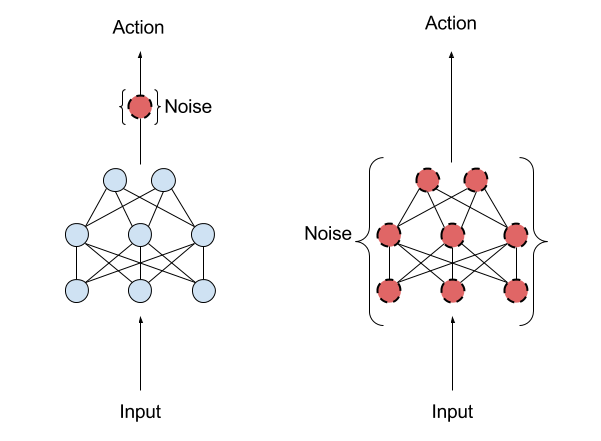
\includegraphics[scale=0.5]{fig/perturbations.png}
\caption{Action vs. parameter space noise}
\end{figure}

When is necessary to explore action space near to some specific action or include momentum of environment, it is possible to use Ornstein-Uhlenbeck random process. \citep{lilicrap2015}. 
\begin{equation}
\hat{A_t} = \mu^\theta(S)  + \nu (\rho - \mu^\theta(S)) + \phi \mathcal{N}(0, 1),
\end{equation}
where $nu, \phi \in [0, 1]$ are constants of the random process and $\nu$ is mean value around which we want to explore the action space. 